\documentclass[13pt,a4paper]{article}
\usepackage[utf8]{inputenc}
\usepackage{vietnam}
\usepackage{geometry}
\usepackage{graphicx}
\usepackage{indentfirst}
\usepackage{minitoc-hyper}
\usepackage{amsmath}
\usepackage{amsfonts}
\usepackage{amssymb}
\usepackage[hidelinks, unicode]{hyperref}
\geometry{letterpaper}
\title{\textbf{ĐỒ ÁN MÔN HỌC}}
\author{Luong Khanh Loc - Bùi Trọng Nghĩa}
\begin{document}
\pdfbookmark{\contentsname}{content}
\tableofcontents
\maketitle
\section{Khoan dưới cân bằng}
\subsection{Tổng quan}
	Trong quá trình khoan một giếng, khi gradient áp suất trong giếng được giữ nhỏ hơn gradient áp suất vỉa thì được gọi là quá trình khoan dưới cân bằng và phương pháp này khác với các phương pháp khoan truyền thống. Trong khi khoan giếng có thể dễ dàng bị ``Kick'' do áp suất dung dịch tuần hoàn dưới đáy giếng luôn nhỏ hơn áp suất vỉa. Tuy nhiên, khi sử dụng phương pháp này, tốc độ khoan được tăng lên khá nhiều đồng thời cũng tránh được hiện tượng mất dung dịch trong khi tuần hoàn. 
\subsection{Những kỹ thuật trong khoan dưới cân bằng}
	Khi khoan áp suất trong giếng nhỏ hơn áp suất trong vỉa nên dễ tạo điều kiện xảy ra hiện tượng “Kick”. Tỉ trọng dung dịch khoan, hay tỉ trọng cột dung dịch là thông số dầu tiên cần xét đến khi muốn hạn chế hiện tượng “Kick”, đồng thời tỉ trọng cũng là một thông số giúp ổn định thành giếng. Vì vậy, việc lựa chọn kĩ thuật khoan cho phương pháp khoan dưới cân bằng là cực kỳ quan trọng. Một số kĩ thuật được đưa vào thực tế như:
	\begin{itemize}
		\item Khoan bằng khí khô
		\item Khoan bằng khí nitơ
		\item Khoan bằng khí tự nhiên 
		\item Khoan bằng khí mù
		\item Khoan bằng bọt
		\item Khoan bằng bọt sánh
		\item Khoan bằng khí hóa lỏng
		\item Flow drilling
		\item Snub drilling
	\end{itemize}
\subsection{Những ưu điểm và hạn chế khi sử dụng phương pháp khoan dưới cân bằng}
	\textbf{Ưu điểm}
	\begin{itemize}
	\item Không sử dụng tác động cơ học để tạo lực đẩy cần thiết cho dung dịch đi vào thành hệ, vì vậy sẽ hạn chế được mất dung dịch trong kể cả khi khoan ở những tầng vỉa có độ thấm cao.
	\item Giảm được thiệt hại đến thành hệ do áp suất trong giếng luôn nhỏ hơn áp suất thành hệ, giúp cho việc giảm chi phí và tiết kiệm thời gian khi kích thích giếng lúc bắt đẩu khai thác. 
	\item Giúp cho việc tìm kiếm các vỉa sản phẩm dễ dàng, nhanh chóng hơn so với phương pháp khoan truyền thống.
	\item Giảm hiện tượng kẹt cần do chênh áp bởi vì không có lớp filter cake ở thành giếng.
	\item Tốc độ khoan được cải thiện hơn so với các phương pháp khoan truyền thống do áp suất ở đầu chòong khoan thấp, đồng thời cũng kéo dài tuổi thọ của chòong khoan.
	\item Cuối cùng, không cần thiết phải xử lý dung dịch khoan nguy hại vì quá trình không sử dụng các loại dung dịch khoan theo kiểu truyền thống.
	\end{itemize}
	\par
	\textbf{Hạn chế}
	\begin{itemize}
	\item Giá thành cao, tùy thuộc vào loại dung dịch.
	\item Việc duy trì điểm dưới áp suất cân bằng thường khá khó khăn. Không có lớp filter cake, khi áp suất đột ngột vượt lên trên mức cân bằng thường gây ra nhiều thiệt hại.
	\item Vấn đề an toàn cũng cần được xem xét cẩn thận, vì khi thực hiện khoan dưới cân bằng phải đối mặt nhiều mối nguy hiểm hơn. Cháy, nổ và BLowout thường dễ xảy ra trong khi khoan dưới cân bằng.
	\item Những vấn đề khác như sập thành giếng do áp suất thành hệ lớn, thiết bị dễ bị hư hại do sử dụng những hệ dung dịch phi truyền thống.
	\item Tùy thuộc vào dung dịch sử dụng có khả năng dẫn nhiệt tốt hay kém, nhưng khi giếng thường xuyên nằm trong trạng dẫn nhiệt kém sẽ gây hư hại đến thành hệ.
	\end{itemize}
\section{Kỹ thuật khoan khí khô}
\subsection{Tổng quan}
	Kỹ thuật khoan bằng khí khô được sử dụng để giảm áp suất vùng đáy giếng xuống thấp nhất để có thể tăng tối đa tốc độ khoan. Với những tính chất được thiết kế, sử dụng khí khô giúp làm mát chòong khoan và làm tăng tốc độ vận chuyển mùn khoan. Khí khô không thực hiện công việc ổn định thành giếng đồng thời cũng không ngăn dòng vào từ vỉa, mục đích duy nhất sử dụng khí khô là làm tăng tốc độ khoan nhanh nhất có thể.\par
	Tuy nhiên, khoan bằng khí khô vẫn đem lại một số lợi ích nhất định ngoài việc tăng tối đa tốc độ khoan:
	\begin{itemize}
	\item{Áp suất trong giếng giảm, tránh được hiện tượng mất dung dịch trong khi tuần hoàn.}
	\item{Có thể tìm được những vỉa có tiềm năng về dầu khí nhưng bị lấp đầy bởi nước vỉa hoặc những dung dịch dùng cho khoan trên cân bằng không thể thực hiện được.}
	\item{Bảo vệ được những tầng sản phẩm nhạy cảm trong vỉa cát chặt sít, vỉa sét nén, vỉa than.}
	\end{itemize}
\subsection{Thiết bị khoan}
\subsubsection{Đầu xoay}
	Để có thể áp dụng kỹ thuật khoan bằng khí cần phải có một thiết bị được gọi là thiết bị kiểm soát khoan xoay ở áp suất thấp (RCD). Trong khi vận hành khoan việc dự tính áp suất giãn nở của khí là không cần thiết vì áp suất trong khoảng không vành xuyến đã đủ để cho khí có thể giãn nở. 
	\begin{figure}[h]
	\centering
	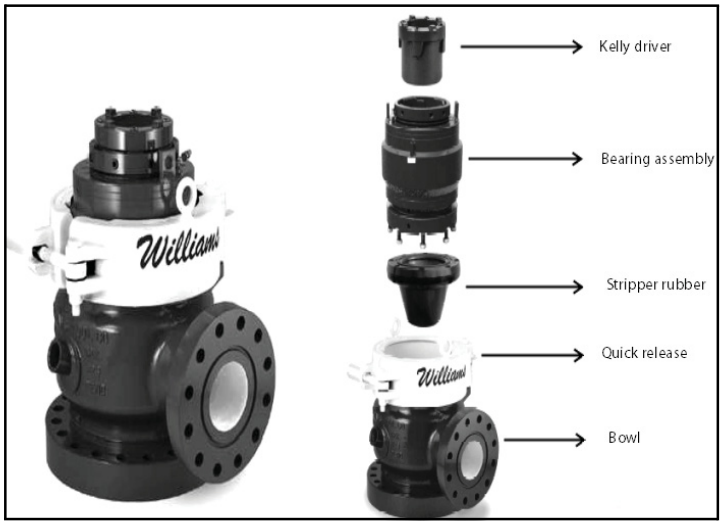
\includegraphics[scale=.7]{Figs/Fig2.PNG}
	\caption{Thiết bị kiểm soát khoan xoay áp suất thấp, $250 psi$}
	\end{figure}
\subsubsection{Bit float và String float}
	Trong chuỗi cần khoan cần có một thiết bị được gọi là Bit float được lắp đặt gần chòong khoan có chức năng giữ cho dòng trong giếng có thể chảy ngược về và bùn tại đáy giếng không bị kẹt lại. Bên cạnh Bit float còn có String float được lắp đặt ở phần đầu của chuỗi cần khoan có chức năng giữ cho áp suất trong toàn bộ chuỗi cần khoan không bị sụt giảm và tạo ra kết nối giữa các bộ phận.
\subsubsection{Fire float và Fire stop float}
	Ở một số quốc gia Fire float và Fire stop float được lắp đặt vào trong cần khoan ở phía trên cảu Bit float. Được sử dụng ở những vùng không chắc chắn về sự có mặt của Condensates trong giếng, thứ có thể trở thành nguyên nhân gây ra hiện tượng Downhole-fires. Trong trường hợp giếng có Downhole-fires, đai an toàn sẽ bị nóng chảy ra cho phép ống lót bịt kín cần khoan để có thể hạn chế được nguồn Oxy đi vào khu vực bị cháy. Quá trình này đồng thời làm tăng áp suất máy nén chính để mở máy nén nhánh.
	\begin{figure}[h]
	\centering
	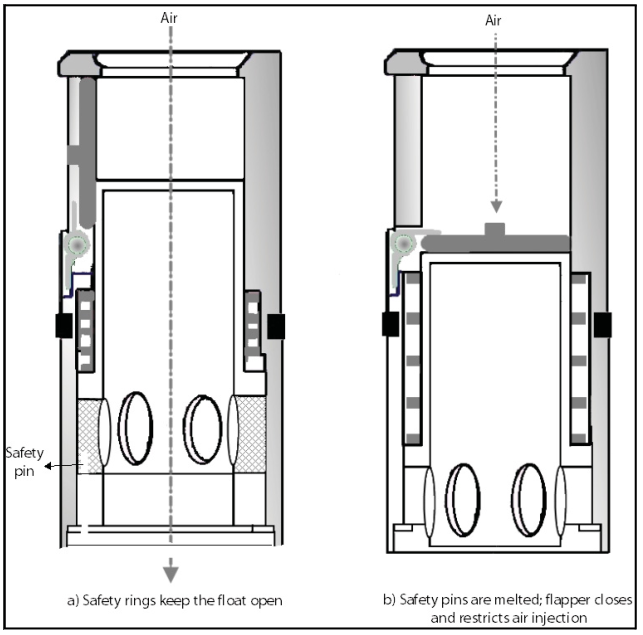
\includegraphics[scale=0.7]{Figs/Fig3.PNG}
	\caption{Fire float và Fire stop float}
	\end{figure}{}
\subsubsection{Ống tháo cạn}
	Chiều dài ngắn nhất cần thiết để có thể sử dụng được ống tháo cạn vào khoảnh 200 đến 300 ft và diện tích mặt cắt ngang ít nhất phải bằng diện tích phần trên của khoảng không vành xuyến. Ống tháo cạn phải được đặt sao cho không bị đẩy lên bởi ảnh hưởng của khí hoặc dung dịch lỏng, đồng thời tránh trường hợp bị xoắn hoặc bị bẻ cong. Nếu áp suất trong ống tháo cạn thấp hoặc bằng áp suất khí quyển, việc đặt van đóng áp ở phía dưới cùng của ống là không cần thiết. Khi cần dừng việc tháo cạn nên đóng van trong đường áp suất cao hoặc ngay tại đầu giếng. Trong một số trường hợp, hai hoặc ba ống sẽ được đặt để đảm bảo sự thông gió của giàn.
\subsubsection{Bình tách, máy khử bụi, bộ giảm âm}
	Chức năng của những thiết bị này có thể được kết hợp chung vào một thiết bị duy nhất. Bụi có thể được kiểm soát bằng dòng nước trong ống tháo cạn và được làm lắng đọng như là bùn ở sàn rung. Những bình tách hay hay máy khử bụi cỡ lớn có thể hoạt động như một máy giảm âm để có thể triệt tiêu sóng âm trong ống tháo cạn.\par
	Hiện nay đã có nhiều giàn và các hệ thống thương mại được lắp đặt để có thể kiểm soát cổng xã của ống tháo cạn. Việc loại bỏ tích tụ tĩnh điện ở những hệ thống bình tách, máy khử bụi, máy giảm âm là cực kì quan trong, vì vậy những hệ thống này thường có một đầu được nối đất.\par
	Hầu hết trong kỹ thuật khoan bằng khí, lượng khí đều thoát ra theo ống tháo cạn, trừ khi lượng khi cần thiết để kiểm soát bui, sóng âm, hay tách dầu từ khí tự nhiên. Sử dụng bình tách kín sẽ an toàn hơn các loại bình tách khác, bìn kín sẽ tránh được hiện tượng va đậm giữa các phân tử bụi, khí và nước là nguyên nhân chính gây tĩnh điện trong các bình chứa.
\subsubsection{Hệ thống bơm khí}
	Khí được bơm vào ống góp phải khô và có nhiệt độ xấp xỉ nhiệt độ môi trường. Nếu sử dụng khí có nhiệt độ quá cao sẽ gây ảnh hưởng đến hệ thống ống quay dẻo, nếu khí ẩm sẽ làm cho khí khó được làm sạch. Vì vậy, hầu hết các máy nén khí hay máy tăng áp đều có một cấp làm lạnh và làm khô khí ở đầu ra.\par
	Trước khi được đưa vào sử dụng, các thiết bị như ống mềm dẫn khí từ máy nén hoặc máy tăng áp cần được thử áp suất ít nhất hai lần để có thể đảm bảo an toàn. Những vị trí như ống dẫn khí hoặc ống mềm từ máy nén áp suất tới ống góp của giàn khoan thường có nguy cơ lớn dẽ bị phá hủy do áp suất vượt quá tải. Khi trong ống dẫn chưa đầy khí nén, nếu ống bị vỡ tại các vị trí kết nối hay chia dòng, ống dẫn thường bị rung với một lực khá lớn. Ống dẫn cần được đặt cố định, đồng thời tại các vị trí kết nối cần có thêm đai an toàn.
\subsubsection{Bơm sương}
	Bơm sương là một thiết bị quan trọng trong hệ thống vận hành. Hai loại bơm thường dùng nhất là bơm sử dụng động cơ diesel và động cơ điện. Công suất của bơm thường nằm trong khoảng 0.5 gpm (2 l/m) tới 5 gpm (20 l/m), áp suất tạo ra lên tới 2,000 psi (14,000 kPa). Hệ thống động cơ bao gồm khớp ly hợp và bộ truyền động giúp cho bơm có thể làm việc ở áp suất cao hơn bình thường, ví dụ như áp suất cần thiết trong ống cuốn xoắn vào khoảng 5,000 psi.\par
	Hệ thống bơm sương cần có hai bể chứ nơi mà chất khử phụ gia và chất hóa học có thể được trộn với nhau để có thể tạo thành hỗn hợp bơm. Kích thước của bể tùy thuộc vào giếng, nhưng lượng dung dịch trong bể phải đảm bảo đủ đê hoạt động được ít nhất một giờ, vào khoảng 6 bbl hay 1 $M^3$. Phía bên trong bể thường có thước đo để định mức dung dịch trong bể.\par
	Khi khoan ở những vùng sa mạc hay những vùng có nguồn nước sạch khan hiếm, sương cần được làm sạch và xử lý độ cứng và các vi sinh vật trước khi đưa vào sử dụng. Nước cứng có thể để lại phần cặn bên trong cần khoan, trong một vài trường hợp có thể gây kẹt cần khoan.\par
	Nước nhiễm bẩn có thể gây ra một số vấn đề như tác động ăn mòn hóa học lên ống chống và cần khoan. Nước biển hoặc nước mặn có thể gây ra ăn mòn hóa học và làm giảm hiệu quả của các chất phụ gia khử sương.
\subsection{Phương pháp vận hành}
\subsubsection{Tuần hoàn dung dịch}
	Hầu hết khi sử dụng kỹ thuật khoan bằng khí khô vào một giếng nào đó, giếng đó sẽ được tháo tải. Cách dễ dàng nhất để tháo tải là thực hiện bơm khí từ phía dưới cùng của ống chống. Thực hiện quá trình này như sau: Sử dụng máy nén để tăng áp suất lên gần cực đại sau đó bơm đồng thời nước và khí cho đến khi áp suất bắt đầu giảm thì ngừng bơm. Thực hiện lại quá trình này cho đến khi giếng ngừng tải. Tỉ trọng trung bình của nước trong cần khoan tăng và áp suất máy nén giảm. Khi một phần của giếng bắt đầu ngưng tải, áp suất nén được giảm xuống.
\subsubsection{Làm khô giếng}
	Trong quá trình làm khô giếng, những phụ gia như chất tẩy khô, chất kiểm soát pH (KOH) hay chất ứng chế hơi nước được đưa vào giếng. Một số phương pháp khác có thể làm khô giếng là đưa khoảng một lít chất phụ gia hấp thụ nước, hơi nước xuống giếng trong khi đang tuần hoàn khí khô, hoặc đóng ram trong BOP và đưa áp suất lên khoảng 1000 psi, sau đó mở ram để nước trong giếng tự phun trào ra ngoài.\par
	Sau một vài giờ đưa khí khô vào giếng, giếng cần tiếp túc được khoan tiếp để có thể làm khô những phần ẩm còn lại trong giếng và ống chống. Ở giếng thân trần, việc làm khô giếng có rất nhiều khó khăn, hầu hết là bởi vì độ nhám của thành giếng.
\subsubsection{Vận hành}
	Trong giếng không còn dung dịch làm đệm cho sự dịch chuyển của cần khoan, đồng thời những vấn đề cso thể xảy ra bởi sự không thích hợp của tỉ trọng dung dịch tương đương. Bắt đầu khoan, đưa chòong khoan vào trong giếng, mở chốt trong của cần khoan. Bên cạnh những vấn đề nguy hiểm có thể xảy ra trên bề mặt, cần khoan có thể bị tuột nhanh ở trong giếng do không còn dung dịch đệm và có xu hướng bị xoắn lại khi xuống tới đáy. Vấn đề này thường khá khó để xử lý. Để hạn chế vấn đề này, khi khoan cần phải sử dụng khí ít nhất một lần ở khớp nối đáy để tránh trường hợp chòong khoan bị cắm sâu vào trong lớp bùn dưới đáy.\par
	Khí trong giếng thường có xu hướng tạo ra các rãnh dạng lỗ khóa và các lát đá mỏng trừ ở những giếng đã chống ống. Để tránh trường hợp cần khoan bị kẹt trong các rãnh dạng lỗ khóa, tốc độ thả cần khoan cần được giảm xuống ở một mức nhất định phù hợp với từng giếng.\par
	Các mối nối giữa các đoạn cần khoan thường bị hư hại khi thực hiện doa trong các đoạn giếng kích thướng nhỏ bởi vì lực xoắn thường lớn nhất ở vị trí các mối nối. Doa với chòong khoan ba chóp xoay cũng có thể làm xoắn thắt lại các bộ phận đỡ hoặc làm mòn chòong khoan ở những vị trí kích thước giếng nhỏ. Hiện tượng này xảy ra với mọi loại chòong khoan trong thành hệ cứng. Vì vậy, trước khi đưa chòong khoan vào giếng cần chắc chắn rằng kích thước giếng đủ rộng đối với chòong khoan.
\subsubsection{Kết nối}
	Ở những vị trí kết nói, giếng cần được tuần hoàn liên tục cho đến khi lượng mùn khoan giảm đến mức thấp nhất. Tại vị trí giếng có kích thước nhỏ, qua trình này thường không kéo dài quá mười phút. Nếu giếng có nhiều khe nứt, bề mặt thành giếng gồ ghề, thời gian làm sạch thường mất khoảng nửa giờ. Khi ngưng tuần hoàn, mùn khoan thường rơi ngược trở lại vào đáy giếng và tích tụ thành bùn ở các vị trí kết nối làm tăng thời gian làm sạch giếng ở những vị trí kết nối.\par
	Lực kéo tác động lên những vị trí kết nối thường phải được giảm đến thấp nhất. Không bao giờ được tác động lực kéo mạnh lên cần khoan nếu khoan ở vỉa khí ít thấm, quá trình cần được thực hiện từ từ. Nếu mùn khoan tích tụ nhiều xung quanh chòong khoan và cần nặng thường làm tắc thậm chí làm cho thành hệ càng bị nén chặt hơn. Nếu xuất hiện các vết nức dạng chìa khóa, quá trình nén chặt sẽ diễn ra nhanh hơn. Trong những giếng bị tắc, cần phải tuần hoàn khí liên tục và di chuyển cần khoan cho đến khi hết kẹt. Nếu không thành công, có thể áp dụng phương pháp đạp. 
\subsubsection{Làm sạch giếng}
	Nếu vận tốc khí ở khoảng không vành xuyến thấp, quá trình ``tắc nghẽn'' (choking) sẽ xảy ra ở những vị trí mùn khoan không được vận chuyển hoặc lơ lửng không thể thoát ra khỏi giếng. Bằng cách giảm áp suất máy nén cho đến khi vận tốc trong khoảng không vành xuyến tăng đến khi đủ khả năng có thể vận chuyển mùn khoan ra khỏi giếng. Đông thời khả năng vận chuyển mùn khoan còn phụ thuộc rất nhiều vào kích thước mùn khoan.\par
	Trong thực tế, kích thước mùn khoan phụ thuộc vào kích thước răng của chòong khoan, với chòong khoan có kích thước răng lớn, dài thường tạo ra mùn khoan kích thước lớn và cũng dễ gây ra hiện tượng ``Choking'' cho đến khi mùn khoan lại tiếp tục bị phá vỡ bởi dòng khí tuần hoàn. Mùn khoan có kích thước nhỏ giúp cho việc tăng tốc độ khoan và tăng khả năng làm sạch giếng của dung dịch khoan.
\subsection{Downhole fires}
	Sự cháy tức thời của hỗn hợp các Hydrocarbon nhẹ trong áp suất khí quyển có thể gây ra hiện tượng Downhole fires. Khi có mặt sự xuất hiện của Oxi trong hỗn hợp Hydrocarbon lỏng, khả năng gây cháy là rất lớn, nếu hỗn hợp đạt tới nhiệt độ cháy, Downhole firs có thể xảy ra. Downhole fires sẽ xảy ra tuần tự theo:
	\begin{itemize}
		\item Đầu tiên, có sự tích tụ của mùn khoan ở những vị trí có vận tốc dòng thấp, thường là ở phần cao nhất của cần nặng hoặc ở vị trí bị sói mòn do tuần hoàn dung dịch trong khoảng không vành xuyến.
		\item Hình thành đai bùn (mud rings). Khi có sự xuất hiện của dòng vào ở trong giếng, mùn khoan có thể sẽ gây bít kín xung quanh cần khoan hay thành giếng (ở những vùng có vận tốc dòng thấp).
		\item Hình thành các hang hốc kín xung quanh cần khoan, ở phía dưới vùng bị bít kín do mùn khoan.
	\end{itemize}
	Nếu khí tiếp tục được tuần hoàn trong khoảng không vành xuyến, làm tăng áp suất trong các hang hốc kín. Khi áp suất tăng, khí trong các hang hốc bị nén lại làm tăng nhiệt độ đến mức có thể gây cháy. Sự xuất hiện của hỗn hợp hydrocarbon lỏng chứa Oxi sẽ là tác nhân cuối cùng gây ra hiện tượng Downhole Fires. 
\subsection{Hệ thống tuần hoàn ngược}
	Trong hệ thống tuần hoàn ngược, dung dịch khoan đi xuống giếng thông qua khoảng không vành xuyến và đi lên bên trong cần khoan đến của hút của máy bơm rồi được đưa vào bình chứa. Mùn khoan được đưa lên bên trong cần khoan thường có kích thước nhỏ hơn so với mù khoan trong khoảng không vàn xuyến. Phương pháp này thích hợp với những giếng có môi trường địa chất nhiệt độ cao và những giếng khoan khí. Sử dụng khí sẽ cho khả năng khoan được sâu hơn. Mực dung dịch trong khoảng không vành xuyến thường được giữ gần bằng với bề mặt.
	\begin{figure}[h]
		\centering
		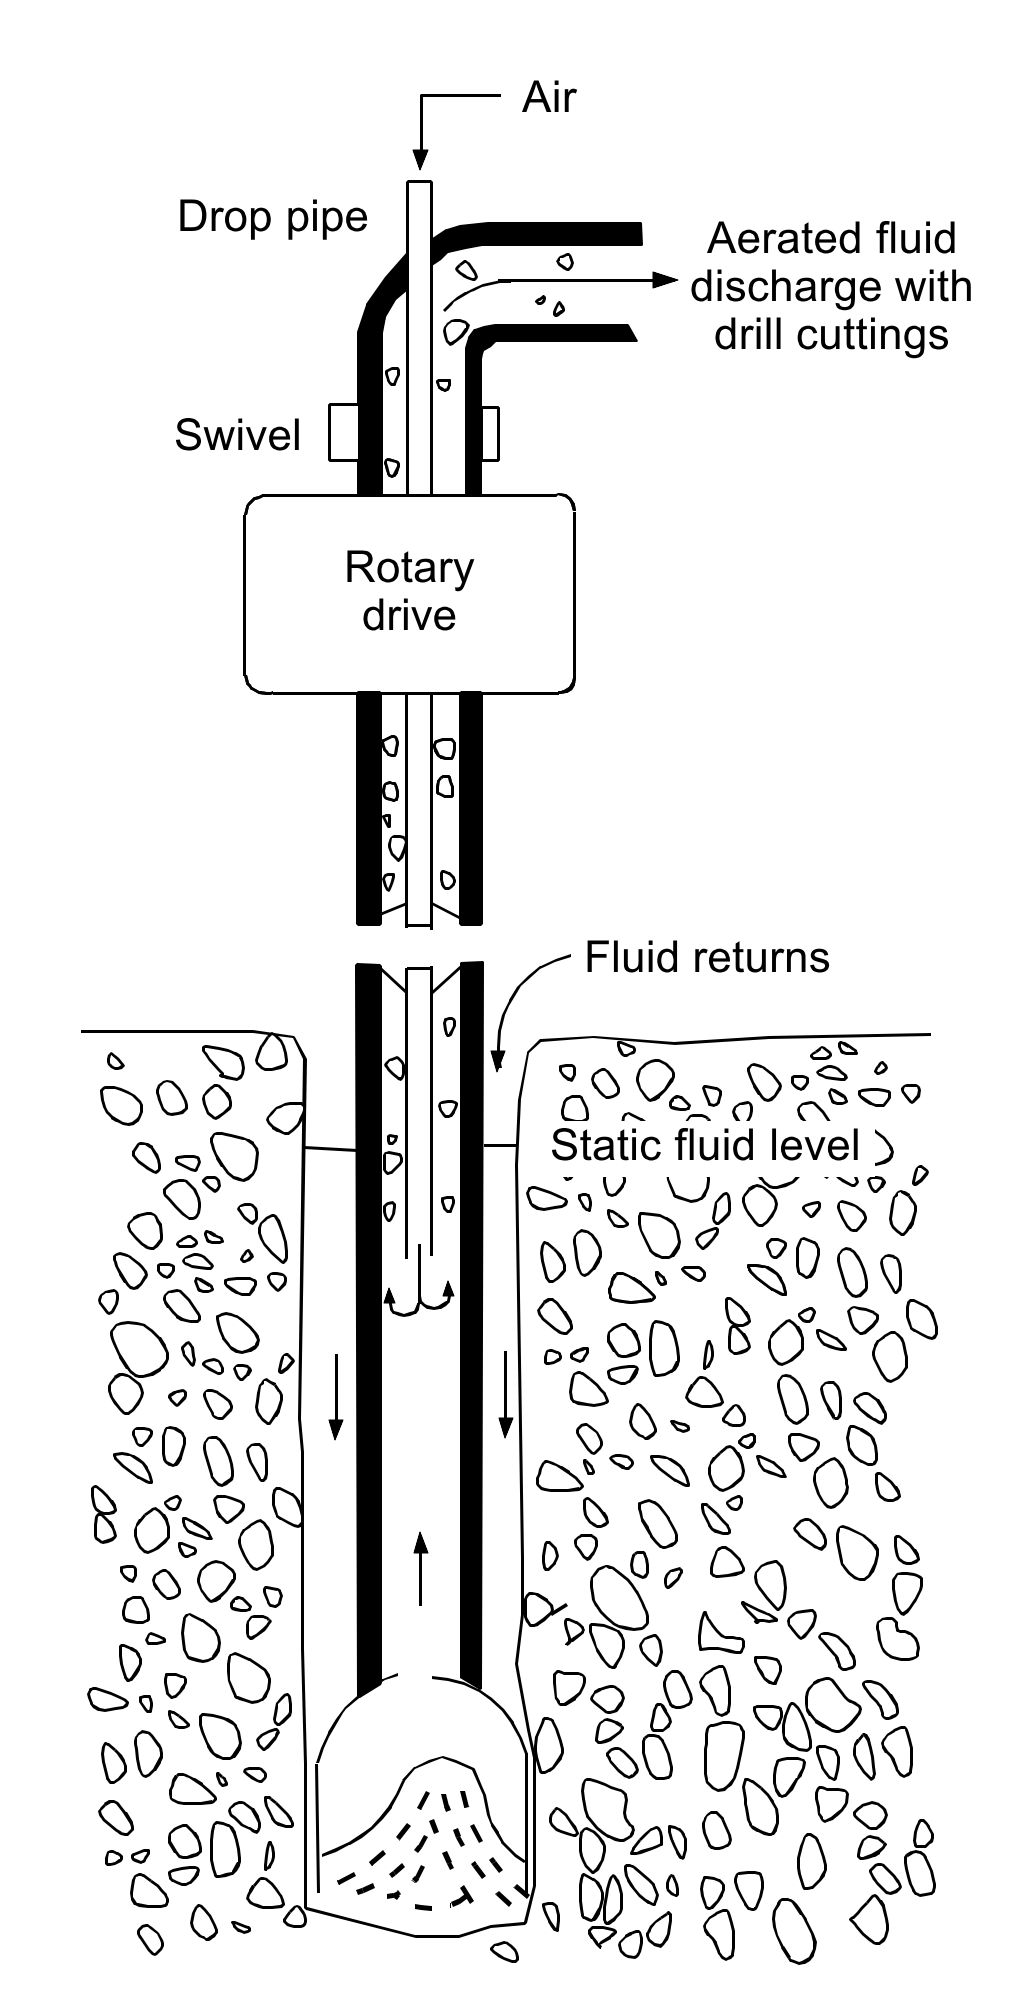
\includegraphics[scale=0.2]{Figs/Fig4.png}
		\caption{Hệ thống tuần hoàn ngược}
	\end{figure}
	Hệ thống tuần hoàn ngược mang lại nhiều lợi ích như:
	\begin{itemize}
		\item Giảm tốc độ của dung dịch trong khoảng không vành xuyến, vì vậy có thể hạn chế được vấn đề sói mòn thành giếng.
		\item Tăng tốc độ cảu dung dịch trong khoảng không vành xuyến, làm giảm thời gian vận chuyển mùn khoan, tăng chất lượng của mùn khoan được lấy mẫu.
		\item Giảm tác động của dung dịch khoan lên thành hệ.
	\end{itemize}
	Đồng thời cũng có một số giới hạn như:
	\begin{itemize}
		\item Mất mát dung dịch thường xảy ra nhiều ở những tầng có độ thấm cao. Tuy nhiên có thể hạn chế tối thiểu lượng dung dịch mất bằng cách thiết kế một chương trình khoan phù hợp.
		\item Khi mực dung dịch trong khoảng không vành xuyến ngang với bề mặt, nó ngăn cản sự xâm nhập của các nguồn địa nhiệt dưới áp suất vào trong giếng khoan gây khó khăn trong công tác đo đạt sự thay đổi của nhiệt độ hoặc hóa chất.
		\item Khi một số dung dịch địa nhiệt xâm nhập được vào giếng, nó làm thay đổi tính chất hóa học của dung dịch khoan, đồng thời có thể loại bỏ một số phụ gia đặc biệt trong dung dịch.
	\end{itemize}
	\par
	Một kĩ thuật thường dùng cho hệ thống tuần hoàn ngược là sử dụng cần khoan 6 in hoặc lớn hơn kết hợp với một máy bơm li tâm hoặc máy phun. Phương pháp này giới hạn cho giếng có đường kính từ 16 in trở lên, sử dụng tool joints có mặt bích đường kính 10 in trở lên để đảm bảo sự tuần hoàn của dung dịch trong giếng. Đối với những vỉa mỏng, không cố kết thường có xu hướng bị xói mòn, đôi lúc tạo ra những hang hốc nhỏ xung quanh mặt bích. Điều này gây khó khăn cho quá trình trám xi măng sau khi chống ống. Vì vậy, phương pháp này thường không được áp dụng cho những giếng có nguồn địa nhiệt không ổn định ngoại trừ một số giếng lớn có sử dụng bơm nhiệt.\par
	Một số kĩ thuật mới được sử dụng cho phép khoan những giếng có đường kính nhỏ sử dụng chòong ba chóp xoay, tăng khả năng khoan sâu và tốc độ khoan. Giảm thời gian tiếp cần hoặc kéo cần ra khỏi giếng.\par
\section{Kỹ thuật khoan bằng khí mù}
\subsection{Tổng quan}
	Khoan bằng khí mù là một phần trong kỹ thuật khoan bằng khí. Khi muốn tăng khả năng vận chuyển mùn khoan và ngăn chặn hiện tượng "mud rings" ở thành hệ, người ta thường chuyển từ khoan bằng khí sang khoan bằng khí mù.\par
	Tỉ lệ nước khí phải tỉ lệ thuận với nhau để mang lại khả năng làm sạch giếng tốt nhất. Sự xuất hiện của nước trong khí làm tăng áp suất giếng. Khí nén cũng làm tăng áp suất giếng và giảm vận tốc dòng khí trong giếng.\par
	Với những giếng dễ bị ảnh hưởng trong khi vận hành, nước (hoặc chất lỏng) sẽ được bơm vào giếng tạo sương để có thể nâng cao khả năng vận chuyển mùn khoan của khí.
\subsection{Vận hành}
	Hầu hết để dừng vận hành hệ thống khoan bằng khí, người ta thường dùng hệ thống khí mù. Bơm một lượng nước vào hệ thống khí đủ để tạo ra sương, trong thực tế, khí mù được đưa vào vận hành chủ yếu để phục vụ hai mục đích chính:
	\begin{itemize}
		\item Phá hủy lớp mud cake được tạo thành từ nước vỉa và mùn khoan kích thước nhỏ trong quá trình khoan ở xung quanh thành hệ.
		\item Vận chuyển được mùn khoan kích thước lớn ra khỏi giếng.
	\end{itemize}
	\par
	\begin{figure}[h]
	\centering
	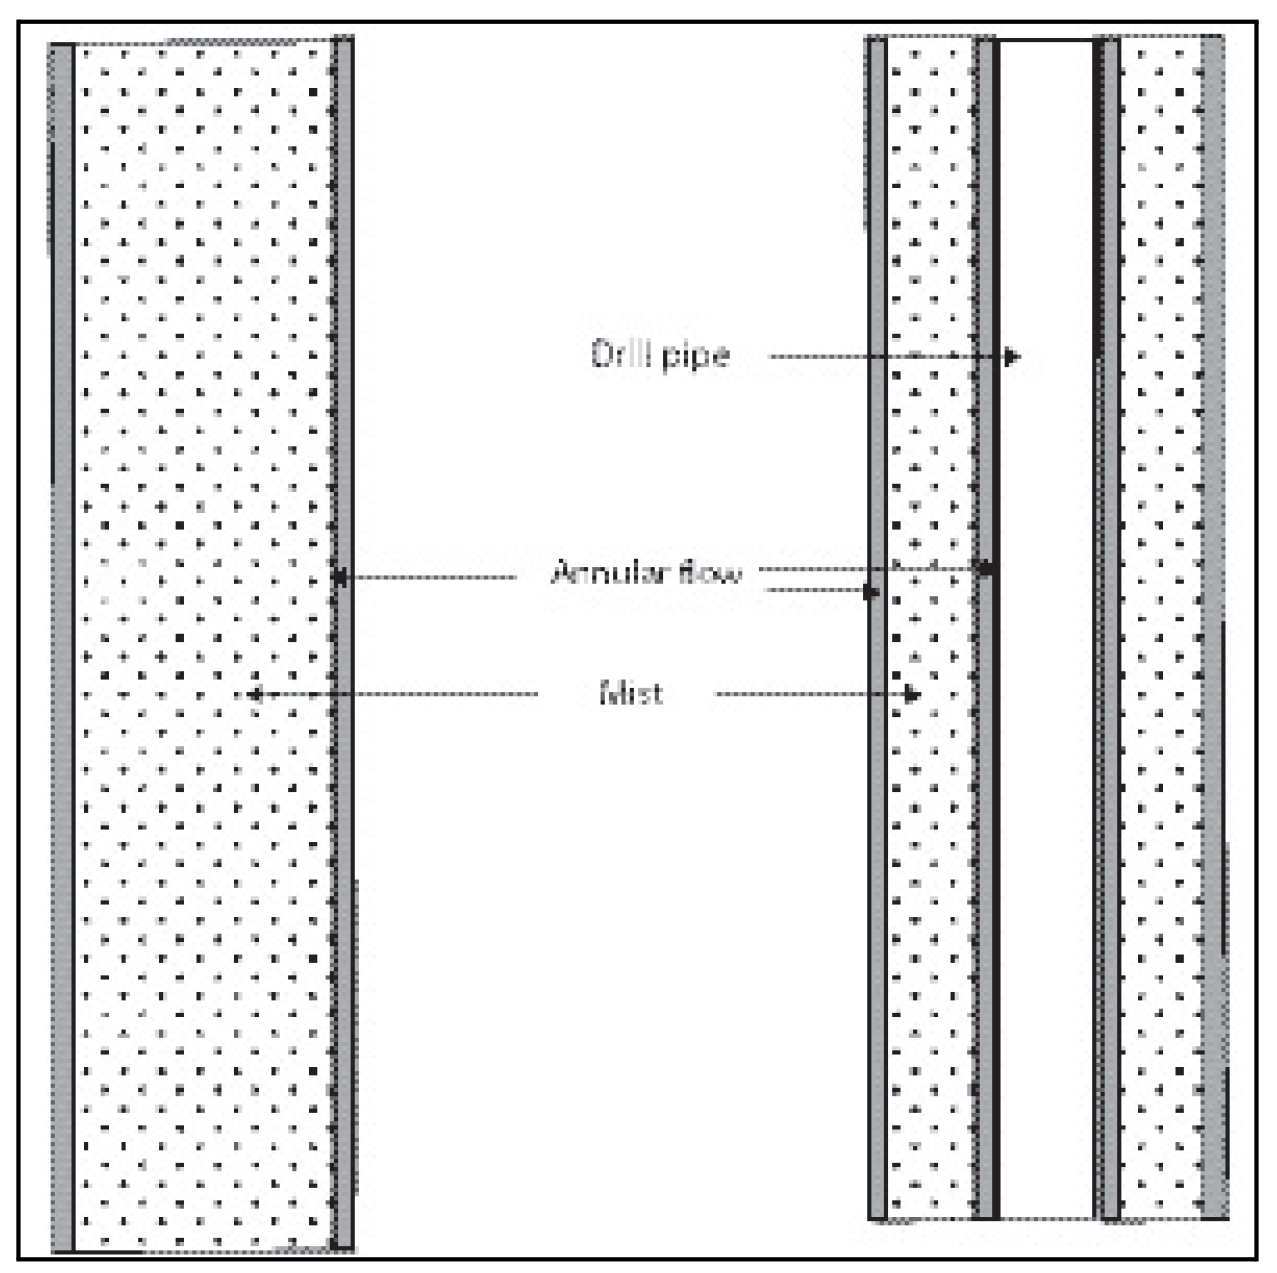
\includegraphics[scale=.3]{Figs/Fig6.png}
	\caption{Khí mù trong và ngoài cần khoan}
	\end{figure}
	\par
	Hình 4 thể hiện quá trình tuần hoàn của khí mù trong khi khoan, pha khí có vận tốc lớn đẩy pha lỏng ra khỏi giếng. Pha khí di chuyển nhanh hơn pha lỏng và tạo ra lực cắt và dòng chảy rối tại bề mặt của lớp nước, loại bỏ các giọt nước nhỏ và mang chúng ra khỏi giếng.\par
	Trong khoan bằng khí mù, chất lượng của khí được giữ ở mức $95\%$ trong điều kiện đáy giếng. Đây là một khá không chính xác, bởi vì trong điều kiện đáy giếng lượng khí còn dư lại phụ thuộc vào kính thước mùn khoan. Tốc độ của pha khí và pha lỏng không bằng nhau, vì vậy việc tính toán thể tích khí và lỏng theo phương pháp thông thường sẽ có độ chính xác không cao. Việc tính toán thường rất phức tạp, sử dụng phương pháp lặp để có thể cân bằng được độ mỏng và lực cắt lên các lớp nước dưới đáy giếng.\par
	Khi ngừng việc bơm khí, các lớp nước bị rơi ngược trở lại xuống đáy giếng cùng với mùn khoan. Sau khi khí được bơm trở lại, sự chênh lệch vận tốc giữa pha khí và pha lỏng được tính toán bằng cách theo dõi khoàn thời gian dịch chuyển giữa thời gian dòng khí và dòng lỏng xuất hiện ở bề mặt.\par
	Hiện nay có nhiều kĩ thuật đưa chất phụ gia tạo bọt vào trong khoan khí mù. Bọt có khả năng làm sạch giếng tốt hơn tại vị trí chòong khoan và cần nặng. Có một vấn đề xảy ra khi thêm chất phụ gia tạo bọt vào dung dịch, đó là bọt có pha lỏng liên tục, khi pha khí trở thành pha liên tục và tạo thành dòng phun ở phần phía trên của giếng sẽ làm giảm khả năng vận chuyển mù khoan đồng thời dễ làm tắc cần khoan. Kĩ thuật sử dụng kết hợp khí mù và bọt là một kĩ thuật mang nhiều ưu điểm đồng thời cũng có nhiều hạn chế, vấn đề cần phải giải quyết.
\section{Kỹ thuật khoan bằng khí tự nhiên}
\subsection{Tổng quan}
	Khoan bằng khí tự nhiên là một trong những kỹ thuật được dùng nhiều nhất cho đến năm 1970 khi giá thành của khí tự nhiên bắt đầu tăng mạnh, không còn phù hợp về mục tiêu kinh tế. Loại khí tự nhiên thường dùng trong kỹ thuật khoan này là metan ($CH_4$). Khí metan có những tính chất phù hợp với các yêu cầu cho một dung dịch khoan loại khí hoặc Gaseated hơn không khí hoặc những loại khí khác. Một số loại khí khác như etan ($C_2H_6$), propan ($C_3H_8$), butan ($C_4H_{10}$) hay một số hydrocarbon khác. Khí tự nhiên trong được dùng trong khoan thường có tỉ trọng 0.8.
\subsection{Ưu điểm}
\subsubsection{Chống ăn mòn}
	Một trong những ưu điểm lớn nhất của việc sử dụng khí tự nhiên là không gây ăn mòn hóa học lên thiết bị lòng giếng, khí tự nhiên không chứa Oxy, vì vậy sẽ không gây ra những vấn đề ăn mòn hóa học. Ăn mòn hóa học trong khi khoan luôn là một vấn đề gây tốn nhiều chi phí, sử dụng khí tự nhiên trong khi khoan sẽ giúp xử lý vấn đề này.
\subsubsection{Down-Hole Fires}
	Vì không chứa Oxy nên khi sử dụng khí tự nhiên có thể tránh được hiện tượng Downhole Fires.
	Khí ở xung quanh miệng giếng và ở dưới sàn khoan có thể gây ra nhiều nguy hiểm, vì vậy cần được thông gió tốt để có thể thoát khí khi lượng khí tích tụ quá nhiều. Khí tự nhiên nhẹ hơn không khí nên thường có xu hướng tập trung nhiều ở đòn quay hoặc những không gian kín tương tự. Hiện tượng này thường xảy ra ở những nơi có khí hậu lạnh, cấu trúc dưới giàn thường dễ bị đóng lại do nhiệt độ.
\subsubsection{Tiện lợi}
	Khi áp suất nguồn khí tự nhiên có thể được gia tăng bằng cách sử dụng đường ống dẫn khí, điều này mang lại nhiều lợi ích cho nhà thầu, nguồn khí thuận tiện hơn, giá thành rẻ hơn so với việc sử dụng máy nén khí.
\section{Kỹ thuật khoan bằng bọt}
\subsection{Tổng quan}
	Khoan bằng bọt là phương pháp sử dụng hệ thống dung dịch khoan bằng bọt, với những ưu điểm như giảm độ nhớt của dầu, tăng khả năng làm sạch giếng. Dung dịch đồng thời giúp giảm bớt mất mát dung dịch vì sự giảm nở của các bọt khí khi chúng được tuần hoàn đến vùng có áp suất thấp. Dung dịch bọt thường có những tính chất sau đây:
	\begin{itemize}
		\item Tăng cường khả năng đưa dầu lên mà không phụ thuộc vào tốc độ.
		\item Khả năng ổn định trong dòng có tỉ trọng thấp.
		\item Ngăn chặn, giảm thiểu mất dung dịch.
		\item Bảo vệ thiết bị khỏi ăn mòn hóa học.
	\end{itemize}\par
	Bọt là một loại dung dịch nhũ tương khi bơm khí vào trong nước (đôi khi là dầu), với nước ở trạng thái liên tục. Những hoạt chất bao quanh mỗi bọt khí giữ cho nó không kết hợp với các bọt khí xung quanh.
\subsection{Khả năng làm sạch giếng}
	Dung dịch bọt có khả năng vận chuyển mùn khoan tốt. Khả năng làm sạch tốt nhất nếu lượng bọt trong dung dịch từ $50\%$ đến $90\%$. Trên $90\%$, dung dịch bọt sẽ chuyển sang pha khí liên tục và mất đi khả năng vận chuyển mùn khoan, dưới $50\%$ sẽ làm giảm khả năng vận chuyển của dung dịch. Trong giếng khoan ngang lượng bọt nằm trong khoảng $30$ – $40\%$ là tốt nhất.
\subsection{Hệ thống thiết bị}
	\begin{figure}[h]
	\centering
	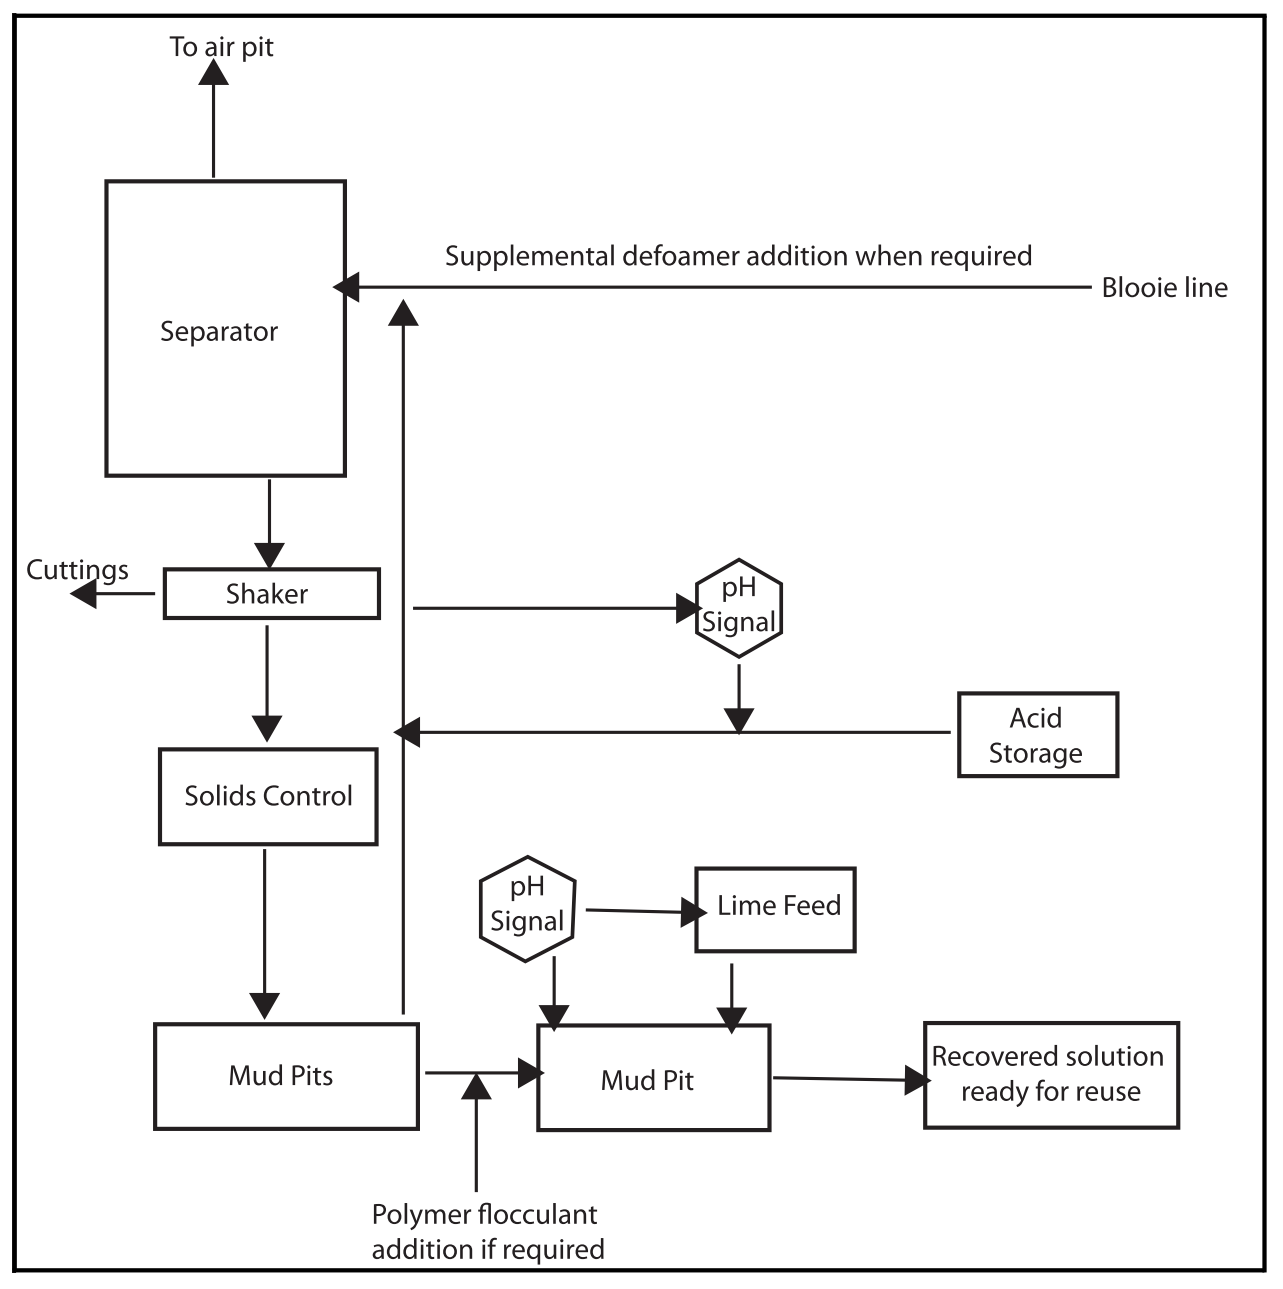
\includegraphics[scale=0.4]{Figs/Fig5.png}
	\caption{Hệ thống thiết bị khoan bằng dung dịch bọt}
	\end{figure}
\subsection{Thành phần dung dịch}
	\subsubsection{Dung dịch bọt gốc nước}
	\textbf{Nước nguyên chất:}\par
	Hầu hết dung dịch bọt đều sử dụng nước là pha liên tục và thường là nước thương mại (nước có thể uống). Mọi sự thay đổi về thành phần đều làm thay đổi giá thành của dung dịch (thường là tăng) và mức độ ổn định của bọt (thường là giảm). Nước nhiễm bẩn cần được xử lí trước khi thêm các phụ gia tạo bọt, đồng thời loại bỏ được các thành phần gây ăn mòn hóa học như các ion âm hay vi sinh vật.\par
	\textbf{Nước biển:}\par
	Được sử dụng ở những khu vực khô hạn khi mà nguồn nước nguyên chất trở nên khan hiếm, nước biển hay nước mặn được sử dụng để làm pha liên tục cho dung dịch bọt. Khi sử dụng nước biển cần sử dụng một số phụ gia đặc biệt để sử lý độ “cường” của nước ($Na^+$, $Ca^{2+}$) thường là soda dư ($NaCO_3$). Tuy nhiên cần phải cẩn thận khi sử dụng soda dư, vì khi sử dụng sẽ dễ dàng hình thành gốc bicarbonate ($HCO_3^-$) gây ra ăn mòn hóa học. Những chất phụ gia đặc biệt này thường khá tốn kém, cần được xem xét trước khi sử dụng.
	\subsubsection{Dung dịch bọt gốc dầu}
	Khi dung dịch gốc nước trở nên nhạy cảm với vỉa (Nhiệt độ cao hay chứa nhiều chất nhiễm bẫn), dung dịch bọt gốc dầu, OleoFoam HT, được sử dụng để quá trình khoan trở nên thuận lợi ở những vỉa nhạy cảm với nước. Dung dịch gốc dầu có khả năng ổn định ở nhiệt độ lên tới $450^oF$, vì vậy thường xuyên được áp dụng ở môi trường có nhiệt độ khắc nhiệt.\par
	Dung dịch bọt gốc dầu (OBFDF, Oil-based foam drilling fluid) thường được sử dụng cho những môi trường đặc biệt, vì vậy cần được thiết ké theo một tiêu chuẩn nhất định. Một số tiêu chuẩn được thiết lập để vận hành trong những điều kiện đặc biệt như tiêu chuẩn của Weatherford:
	\begin{itemize}
		\item Dung dịch gốc cần tương thích với các phụ gia phổ biến như các chất ức chế ăn mòn, cặn.
		\item Mức độ tạo bọt phải lớn hơn 130mL, vòng đời của bọt phải lớn hơn ba phút. Mức độ tạo bọt là thể tích bọt được tạo ra bằng cách trọn chất tạo bọt vào 100mL dung dịch gốc. Vòng đời của bọt được tinha bằng thời gian 50mL dung dịch bọt bị phá vỡ hoàn toàn.
		\item Dung dịch phải tương thích với các thiết bị lòng giếng.
		\item Hệ thống vận hành phải đủ điều kiện để có thể vận hành với mọi loại dung dịch gốc dầu trong bản thiết kế dung dịch khoan.
		\item Dung dịch phải có khả năng tái sử dụng, dung dịch tái sử dụng phải hoạt động tốt.
		\item Dung dịch phải tương thích với quá trình lọc dầu ở các nhà máy lọc dầu để tạo ra những sản phẩm có giá trị thương mại.
	\end{itemize}
	\par
	\textbf{Phụ gia tạo bọt dầu:}\par
	Khi độ ổn định của bọt quá thấp làm cho vòng đời của bọt bị rút ngắn, phụ gia dầu tạo bọt được đưa vào dung dịch. Khi sử dụng phụ gia này pha liên tục thường là dầu thô, diesel, dầu khoáng hay các hợp chất của olefin hoặc este. Dung dịch bọt loại này thường ổn định ở nhiệt độ cao hay những vị trí phức tạp khó giải quyết bằng cách vận hành loại dung dịch thông thường.\par
	Các chất phụ gia kích thích hoạt động bề mặt thường dùng là silicon oligomer, có khả năng thay đổi linh hoạt để tương thích với điều kiện hoặc thiết kế thể tích, vòng đời mong muốn kể cả những vị trí có mật độ bọt thấp.\par
	\textbf{Phụ gia khử bọt:}\par
	Thường sử dụng gốc silicone, khi sử dụng chất khử bọt quy trình tuần hoàn thường là “tạo bọt – khử bọt – tái tạo bọt” và vẫn có thể giữ được tính chất mong muốn ban đầu của dung dịch bọt. Thực tế, hầu hết các chất khử bọt tốt như alcohols, ete, hợp chất hydrocarbon hoặc một số hợp chất khác đều không tương thích với chất tạo bọt gốc silicone hay chất làm tăng độ nhớt.\par
	\textbf{Phụ gia tăng độ nhớt:}\par
	Thường sử dụng một số polime hòa tan trong dầu trên thị trường nhưng hầu hết đều không phù hợp với các công thức tạo dung dịch khoan gốc bọt. Hiện nay, Styrene-Isoprene thường được sử dụng để thiết kế những tính chất mong muốn cho dung dịch bọt. Những hợp chất đồng trùng hợp thường được sử dụng cho môi trường khoan có nhiệt độ cao, tăng độ nhớt của pha liên tục (pha lỏng), cho phép điều chỉnh tính chất bọt tùy thuộc vào điều kiện khoan như vận chuyển mùn khoan hay kiểm soát áp suất đáy giếng.
\subsection{Hạn chế}
	Giá thành, một trong những yếu tố chủ yếu làm tăng giá thành của dung dịch bọt là các chất phụ gia tạo bọt và các hợp chất hóa học có chức năng ổn định và kiểm soát ăn mòn. Giá thành của dung dịch bọt thay đổi theo kích thước giếng, tính chất hóa học cần thiết cho những giếng có nhiệt độ trên $200^oF$ hoặc giếng có điều kiện khai thác khắc nhiệt. Chất tạo bọt hóa học khá phổ biến đối với những dự án lớn, vì vậy chi phí sẽ giảm tương đối đáng kể nếu được mua theo số lượng lớn.\par
	Đối với những giếng có nhiệt độ khắc nhiệt, trên $200^oF$, dung dịch bọt có xu hướng di chuyển như dung dịch khí, làm mất đi khả năng ổn định, kiểm soát áp suất, làm sạch mùn khoan trong giếng.\par
	Trong trạng thái nhũ tương dung dịch bọt khá ổn định, với lớp màng có khả năng chống phá vỡ trong điều kiện vỉa muối nóng, vỉa nước chứa acid. Tuy nhiên, dung dịch bọt có xu hướng bị phân tách trong quá trình tuần hoàn, lúc đó phần dung dịch bị nhiễm bẩn sẽ nhanh chóng bị phá hủy bởi vì dầu nhẹ, khoáng vật nhiệt độ cao hay nước chứa acid đều làm những tác nhân khử bọt tốt. Một số phương pháp giải quyết vấn đề này như:
	\begin{itemize}
		\item Giảm dòng vào bằng cách tăng áp suất bề mặt.
		\item Tăng áp suất đáy giếng bằng cách tăng thể tích lượng nước trong dung  dịch bọt để làm tăng tỉ trọng dung dịch bọt.
		\item Thêm chất phụ gia làm tăng độ ổn định cho dung dịch bọt.
		\item Không tái sử dụng dung dịch bọt, thay vào đo, sử dụng hệ thống tuần hoàn dung dịch đơn.
	\end{itemize}
\section{Kỹ thuật khoan bằng bọt sánh}
	Khoan bằng bọt sánh là một kỹ thuật mở rộng trong kỹ thuật khoan bằng bọt. Kỹ thuật này được sử dụng để khoan vào những thành hệ có độ cố kết thấp, cần dung dịch khoan có tỉ trọng thấp nhưng cần thêm vào các phụ gia có chức năng ổn định thành hệ. Lớp màng của bọt sánh có độ bền cao hơn so với bọt nên có khả năng vận chuyển mùn khoan có kích thước lớn hơn. Khi sử dụng dung dịch bọt sánh, tốc độ dung dịch ở khoảng không vành xuyến tăng từ 100 đến 200 ft/min, vì vậy không cần thiết phải sử dụng hệ thống nhiều máy nén như các loại khí khác.(Có thể thay đổi tốc độ dung dịch tùy thuộc vào lượng chất lỏng chảy vào giếng từ thành hệ.)\par
	Dung dịch bọt sánh được sử dụng để vận chuyển mùn khoan trong những giếng khoan đường kính lớn, trong những thành hệ có độ cố kết yếu. Thành phần của các chất phụ gia trong dung dịch bao gồm bentonit là 10 - 15 lb/bbl, với gôm polisacarit là 0.2 - 0.5 lb/bbl, với soda khan là 1 lb/bbl và một số chất phụ gia tạo bọt khác được đưa vào bằng khoảng 1\% thể tích. Có thể sử dụng bentonit peptit hóa cho bentonit và một số loại pomymer hữu cơ khác cho gôm polisacarit. Dòng dung dịch tuần hoàn ngược trở lại thường có độ nhớt cao hơn so với dung dịch ban đầu do sự có mặt của lớp bùn trong giếng, vì vậy dung dịch bọt sánh phải được bơm vào giếng với tốc độ cao để có thể tạo ra dòng tuần hoàn ngược. \par
	Hệ thống kiểm soát dung dịch bọt sánh cần có một máy bơm thể tích nhỏ để bơm vật liệu tạo bọt vào dòng khí. Ngoài ra còn có thể sử dụng máy tạo bọt để đưa bọt thẳng vào trong đường ống. Thành phần của dung dịch được lựa chọn sao cho có thể cung cấp khả năng ổn định cho dung dịch trong những môi trường khác nhiệt như nước vỉa chứa muối hay trong dầu. Trong những môi trường này bentonit thường không được sử dụng.\par
	Một yếu tố ảnh hưởng đến mức độ hoàn thiện của dung dịch bọt sánh là khả năng duy trì cột dung dịch bọt sánh liên tục từ ống dân bùn khoan đến ống tháo cạn. Áp suất bề mặt, momen xoắn của chuỗi cần khoan, mức độ liên tục và hình dạng bọt của dung dịch tại ống tháo cạn là những yếu tố cần phải xem xét khi thay đổi thành phần và tốc độ bơm dung dịch. Tốc độ khoan và kích thước mùn khoan cũng là những thông số quan trọng cần được xem xét.
\section{Kỹ thuật Snub drilling}
\subsection{Tổng quan}
	Snub drilling là phương pháp kiểm soát sự chuyển động của cần khoan khi ra vào giếng khoan trong khi vẫn tiếp tục kiểm soát giếng. Không giống với những phương pháp khoan và hoàn thiện giếng truyền thống, kĩ thuật này yêu cầu phải sử dụng dụng dịch giảm tỉ trọng, điều này thường làm tăng giá thành giếng khoan, gây hư hại thành hệ.\par
	Hệ thống snubbing có thể trợ giúp quá trình vận hành giàn khoan khi xuata hiện áp suất bề mặt. Bình thường snubbing thường được thực hiện trong khi giếng đang trong trạng thái khoan dưới cân bằng. VÌ vậy, các phương pháp và thiết bị kiểm soát áp suất (thường là BOP) cần được sử dụng để giữ dụng dịch nằm trong tầm kiểm soát.
\subsection{Thiết bị}
	\subsubsection{Hệ thống thủy lực}
	Hệ thống thủy lực được đưa vào sử dụng vì có những ưu điểm như hệ thống điều khiển chuẩn xác bằng tay, hệ thống thủy lực thường nhanh và có phản hồi chuẩn xác trong thời gian tương ứng. Mọi thay đổi về áp suất bằng cách điều khiển van đều được phản hồi gần như ngay lập tức ở mọi vị trí trong hệ thống. Hệ thống thủy lực dùng để điều khiển chuyển động của cần khoan, tubing, ống chống thông qua búa thủy lực, đối áp vành xuyến. Van an toàn dùng để ngăn cản áp suất quá tải. Đặc tính an toàn này có thể loại bỏ những sai sót trong vận hành do con người.
	\subsubsection{Hệ thống Snubbing}
	Hệ thống Snubbing có thể chia thành bốn phần cơ bản như sau:
	\begin{itemize}
		\item Hệ thống thiết bị cơ bản
		\item Cột ống và thành phần cột ống
		\item Hệ thống thiết bị kiểm soát giếng
		\item Thiết bị phụ.
	\end{itemize}
	\begin{enumerate}
		\item Hệ thống Snubbing cơ bản\par
		Hệ thống thiết bị cơ bản thường là những hệ thống thủy lực hay cơ khí được dùng để tạo lực đẩy, kéo, xoắn lên chuỗi cần khoan. Ba loại hệ thống đẩy thường dùng là hệ thống kích thủy lực, hệ thống thủy lực hành trình dài, hệ thống nâng cơ khí ``Rig assist''.\par
		``Rig assist'' và hệ thống kích được sử dụng rất phổ biến trong hệ thống thiết bị Snubbing vì khả năng xử lý được nhiều vấn đề xảy ra với giếng. Kích có thể vận hành được cả trên giàn truyền thống và giàn phi truyền thống.\par
		Những ưu điểm của ``Rig assist'' so với các loại khác như là:
		\begin{itemize}
			\item Hiệu suất cao
			\item Khả năng chịu xoắn tốt
			\item Thiết kế gọn nhẹ
			\item Thích hợp với nhiều loại ống từ $\dfrac{3}{4}$ đến $13\dfrac{3}{8}$ in.
			\item Lực tác động chủ yếu lên đầu giếng, giúp giảm bớt phá hủy thành hệ, mang lại nhiều lợi ích trong khi khoan
			\item Có thể thay đổi trọng lượng của thiết bị để có thể phù hợp với quá trình lắp đặt.
		\end{itemize}
		Hạn chế của ``Rig assist'':
		\begin{itemize}
			\item Thời gian kéo ống và tiếp ống lâu hơn
			\item Quá trình lắp đặt khó khăn
			\item Sử dụng chuỗi cần khoan đơn.
		\end{itemize}
		\begin{figure}[h]
			\centering
			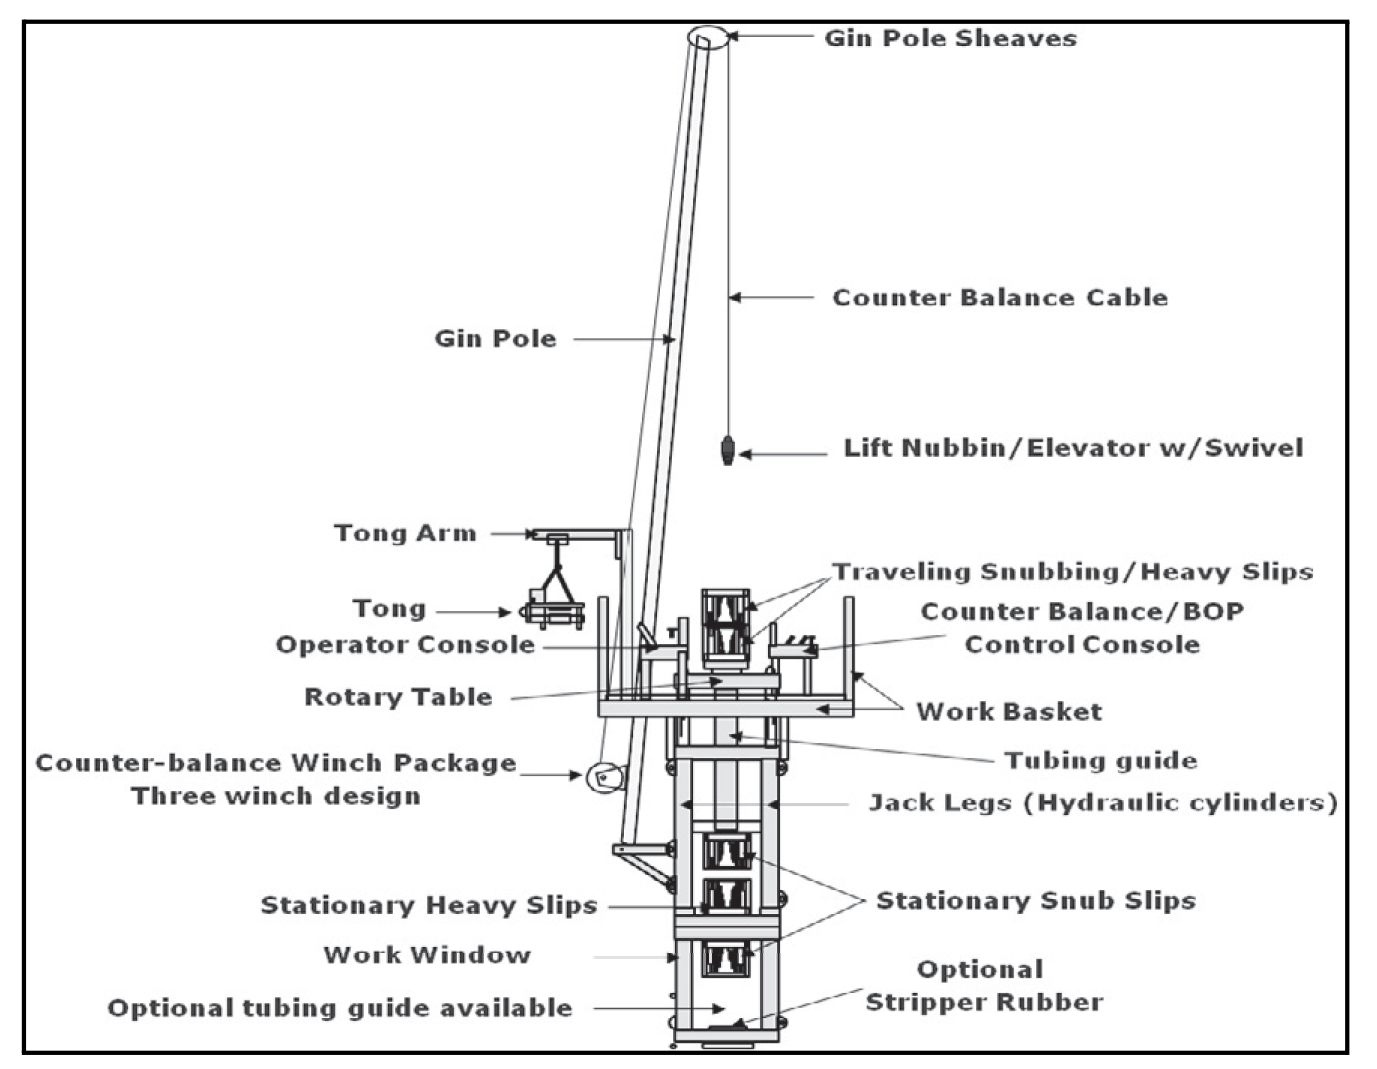
\includegraphics[scale=.3]{Figs/Fig7.png}
			\caption{Hệ thống Snubbing}
		\end{figure}
		\begin{figure}[h]
			\centering
			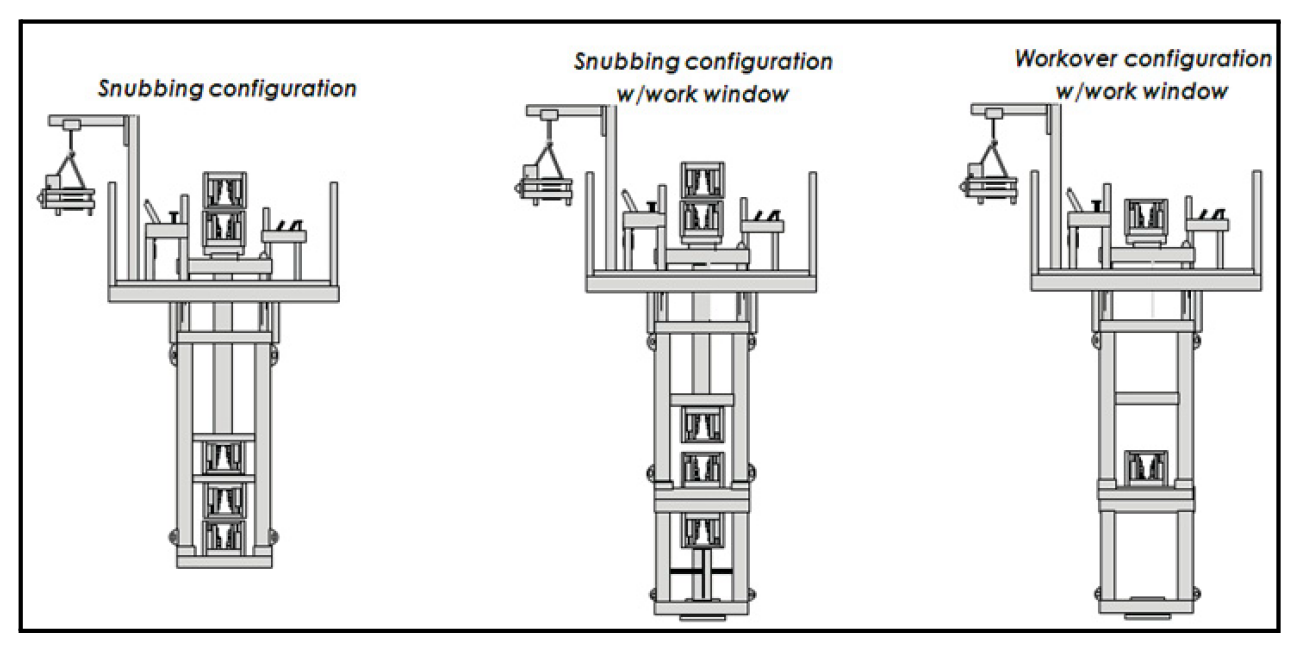
\includegraphics[scale=0.3]{Figs/Fig8.png}
			\caption{Hệ thống Snubbing cơ bản}
		\end{figure}
		\item Thành phần chuỗi cần khoan
		\begin{itemize}
			\item Van đối áp
			\item Stabbing van
			\item BOP
			\item Khớp nối vòng tuần hoàn
			\item Ống tuần hoàn
			\item Ống nối
			\item Bộ khoan cụ và thành phần bộ khoan cụ.
		\end{itemize}
		\item Hệ thống kiểm soát giếng \par
		Hệ thống kiểm soát sơ cấp:\par
		Gồm ba thành phần đĩa cao su, đầu bịt an toàn dạng vòng, ram.\par
		Đĩa cao su được dùng để có lập không gian giữa các bộ phận, loại bỏ hiện tượng ``Ram to ram stripping'' trong những giếng áp suất thấp, rút ngắn thời gian bảo trì trong khi khoan. Có nhiều loại đĩa cao su và thường được lắp đặt ở giá đỡ snubbing.\par
		Đầu bịt an toàn dạng vòng thường được dùng để kiểm soát dung dịch khoan. Ngoài ra còn dùng cho mục đích tháo lắp, nhưng thường chỉ được sủ dụng trong giai đoạn kiểm soát giếng thứ cấp.\par
		Ram và những bộ phận liên quan được sử dụng thường xuyên trong hệ thống snubbing, cho phép kiểm soát di chuyển của ống với áp suất bề mặt. Những bộ phận cơ bản của ram:
		\begin{itemize}
			\item Stripper pipe ram
			\item Hệ thống cuộn cân bằng
			\item Hệ thống xả áp
			\item Van cản dòng.
		\end{itemize}
		\par 
		Hệ thống kiểm soát thứ cấp: \par
		Mục đích của kiểm soát thứ cấp là tiếp tục duy trì kiểm soát giếng trong trường hợp xảy ra vấn đề không mong muốn hoặc trong thời gian bảo trì hệ thống kiểm soát thứ cấp.\par
		Những bộ phận và thành phân của BOP trong bộ kiểm soát thứ cấp thường tùy thuộc vào nhà sản xuất và mục đích sử dụng, bao gồm những bộ phận cơ bản sau:
			\begin{itemize}
				\item Hai ống ram
				\item Một ram đóng, một ram cắt
				\item Đường tiết lưu, đường bơm dung dịch dập giếng.
			\end{itemize}
		\par
		Hệ thống kiểm soát tam cấp:\par
		Mục tiêu của kiểm soát tam cấp là tiếp tục kiểm soát giếng trong trường hợp khẩn cấp hoặc trong thời gian bảo trì hệ thống kiểm soát sơ cấp và thứ cấp. Hệ thống kiểm soát tam cấp bao gồm ram cắt đơn với hệ thống kiểm soát độc lập.\par
		Hệ thống kiểm soát chính được đặt ở work basket, tránh xa miệng giếng khoan để giữ an toàn khỏi rò rỉ khí dễ gây cháy nổ.
		\item Hệ thống thiết bị phụ\newline
		Hệ thống nâng giữ cần khoan và work basket: Được thiết kế nhằm mục đích di chuyển ống ra vào giếng đồng thời lắp đặt để kết nối chuỗi cần khoan ra vào giếng. Hệ thống nâng giữ cần khoan được vận hành trong quá trình vận hành hệ thống HWO/Snubbing:
			\begin{itemize}
				\item Nhận và tiếp cần từ work basket
				\item Tạo lực xoắn lên cần bằng cả hai phương pháp tay và thủy lực
				\item Không cần tháo bỏ các bộ phận kết nối, vòng tuần hoàn, ống tuần hoàn trong quá trình bảo trì.
			\end{itemize}
		Work basket được đảm bảo an toàn bằng cách sử dụng lối vào là một cầu thang, ngoài ra lối thoát hiểm khẩn cấp được lắp đặt. Lối thoát hiểm khẩn cấp được lắp đặt bằng một trong những cách sau:
			\begin{itemize}
				\item Dây cáp geromino
				\item Cánh cháy
				\item Catwalk 
				\item Cầu thang thoát hiểm.
			\end{itemize}
	\end{enumerate}
\section{Kỹ thuật khoan bằng khí Nitơ}
\subsection{Màng Nitơ}
	Màng nitơ được tọa ra bằng cách bơm khí đi xuyên qua một hệ thống màng gồm nhiều hợp chất có khả năng giữ lại phân tử nitơ nhưng cho phép các phân tử khác như oxi, carbon dioxide và phân tử hơi nước đi qua. Một phần phân tử khí oxi bị giữ lại trong màng cùng khí nitơ, lượng khí oxi này tùy thuộc vào áp suất qua màng, áp suất càng lớn thì lượng khí bị giữ lại càng ít. Màng nitơ sử dụng khi muốn hỗn hợp khí có từ 4 đến 5\% khí oxi cộng với các khí khác. 
	\begin{figure}[h]
	\centering
	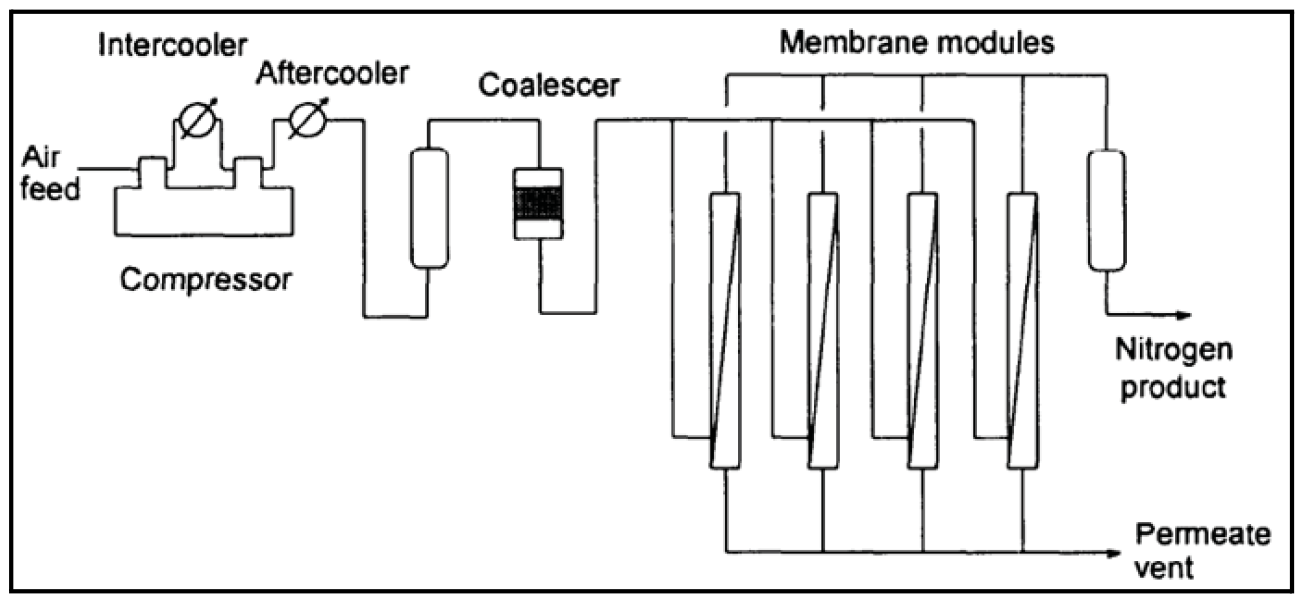
\includegraphics[scale=.5]{Figs/Fig9.png}
	\caption{Hệ thống tạo màng nitơ}
	\end{figure}
	\par
	Hiệu suất của hệ thống tạo màng nitơ (hình 9)  thường là 50\%. Áp suất đầu vào hệ thống màng thường là 350 psi, đầu ra của máy nén khí là 300 psi. Nếu áp suất đầu vào tăng thì hiệu suất của hệ thống sẽ tăng, nhưng hiệu suât của bình và lượng oxi được giữ lại sẽ giảm. Màng nitơ thường khá nhậy cảm với nhiệt độ vì vậy trong hệ thống thường có thêm một bộ biến nhiệt. 
	\subsubsection{Ưu điểm}
		Vì hàm lượng oxi thấp nên khi đi vào bình tách kín màng nitơ khó bị kích thích cháy từ tĩnh điện.\par
		Màng nitơ có thể được sử dụng với dung dịch khoan gốc dầu. Không giống như khí tự nhiên, màng nitơ ít bị hòa tan trong dầu và ít gây ăn mòn hóa học cho hệ thống khoan.
	\subsubsection{Hạn chế}
		Chi phí sản xuất màng nitơ thương khá đắt đỏ vì hiệu suất của hệ thống sản xuất chỉ nằm vào khoảng 50\%, muốn tăng hiệu suất hệ thống thường phải tăng gấp đôi chi phí so với khi sử dụng các loại khí khác.
\subsection{Nitơ lỏng}
	Nitơ lỏng là nitơ nguyên chất được hóa lỏng dưới nhiệt độ -320$^oF$. Nitơ lỏng được vận chuyển đến giàn khoan bằng xe bồn ở trên đất liền, bằng xà lan hoặc bình chứa ở trên biển.\par
	Nitơ được bơm bằng một loại bơm đặc biệt bơm ba bittong với áp suất lên tới 10000 psi hoặc hơn. Sau khi đi qua bơm, nitơ lỏng được gia nhiệt để trở về trạng thái khí hóa lỏng cho mục đích sử dụng.\par
	Nitơ có nhiệt dung riêng thấp, cần khoảng 134000 BTU để có thể sản xuất được 10000 scf khí nitơ từ nitơ ở trạng thái lỏng. Lượng nhiệt này thường có sẵn ở xe vận chuyển, ở những vùng có khí hậu lạnh cần phải dùng tới máy gia nhiệt để có thể cung cấp đủ nhiệt lượng cho việc sản xuất khí nitơ.
	\subsubsection{Ưu điểm}
	Không gây ăn mòn hóa học lên hệ thống khoan: \par
	Nitơ lỏng không chứa oxi vì vậy không hình thành nên môi trường ăn mòn. Tuy nhiên, nó vẫn có khả năng gây ăn mòn ở phần đáy giếng nếu xuất hiện sự có mặt của $CO_2$ và $H_2S$.\par
	Không gây cháy nổ:\par
	Nitơ lỏng nguyên chất không thể làm nguồn gây nổ hay cháy do nó không chứa oxi.Ngoài ra nitơ lỏng có thể hoặc động như một chất chống cháy.\par
	Áp suất cao:\par
	Nitơ có thể được bơm xuống dưới giếng với một áp suất rất lớn do quá trình hóa lỏng đã tạo ra một áp suất cực lớn trước đó. Vì vậy nitơ khá lí tưởng cho kỹ thuật khoan bằng khí.
	\subsubsection{Hạn chế}
	Giá thành:\par
	Hệ thống vận chuyển nitơ lỏng thường rất tốn kém, nitơ lỏng cần phải được chưa trong một loại bình chứa đặc biệt, cần được tăng áp và làm nóng trong quá trình vận chuyển. Chi phí vận chuyển thường nhiều hơn ít nhất gấp năm lần chi phí nén khí và ít nhất gấp hai lần chi phí sản xuất nitơ màng.\par
	Dễ bay hơi:\par
	Nitơ lỏng thường dễ bị bay hơi ở môi trường có nhiệt độ cao, trong quá trình vận chuyển đến giàn khoan.\par
	Chất chống cháy:\par
	Sự có mặt của khí nitơ làm hạn chế sự cháy trong hệ thống cháy. Vì vậy, cần phải có một lượng khá lớn khí tự nhiên để có thể không làm gián đoạn hệ thống cháy.
\section{Kỹ thuật khoan bằng Gaseated Fluid}
\subsection{Tổng quan}
	Gaseated fluid là loại dung dịch khoan có khả năng thay đổi tỉ trọng một cách linh hoạt, là hỗn hợp giữa khí và lỏng mà không có thêm bất cứ một thành phần phụ nào khác như phụ gia tạo nhũ tương hay phụ gia tạo độ ổn định. Hệ thống gaseated được vận hành một cách rất dễ dàng, pha lỏng chỉ cần là một trong những dung dịch có khả năng tương thích vơi hệ thống khoan cả trong khi đóng giếng và mở giếng. Ở pha khí có thể dử dụng khí tự nhiên, nitơ hoặc những khí khác. Việc lựa chọn chất lưu sẽ phụ thuộc và tính chất của hệ thống (khả năng ức chế, độ bền nhiệt, mức độ nhiễm bẩn). Quá trình lựa chọn khí dựa trên mức độ nguy hiểm của khí đó khi ở trên mặt đất, down-holw fire, mức độ ăn mòn hóa học, giá thành và mức độ tiện lợi (ở gần hay xa giàn khoan).
\subsection{Dự đoán áp suất thủy tĩnh}
	Thể tích dung dịch bơm vào giếng có thể được thay đổi một cách linh hoạt khi sử dụng hệ thống gaseated. Tốc độ và thể tích dung dịch mong muốn phụ thuộc vào áp suất thủy tĩnh và tỉ trọng dung dịch tương đương ở phần trên của giếng. Sử dụng tỉ trọng dung dịch tương đương để tăng vận tốc dung dịch ở phần trên của giếng thường không thích hợp đồng thời còn phải phụ thuộc vào chu vi dính ướt và diện tích của khoảng không vành xuyến.\par
	Poettman và Bergman đã phát triển một mô hình dự đoán áp suất thủy tĩnh cho dung dịch gaseated ở điều kiện tĩnh. Hạn chế của phương pháp này là xét đến những điều kiện như ma sát hay ảnh hưởng của sự phân tách dung dịch trong khoảng không vành xuyến.\par
	Để dự đoán áp suất đáy giếng trong khi khoan bằng gaseated có thể sử dụng những mô hình tương quan dự đoán áp suất như tương quan Hagedorn - Brown, tương quan Beggs - Brill. Nếu hệ thống gaseated được giả sử như là một hệ đồng nhất, có thể sử dụng định luật hàm mũ cho hỗn hợp khí-lỏng để tính toán tổn thất áp suất do ma sát trong khoảng không vành xuyến như sau:
	\begin{equation}
	\Delta P = \Delta L f \rho V_a^2/\{21.1(D_h-D_p)\}
	\end{equation}
	Với \par
	$f$ = Hệ số ma sát đạt được bằng cách tính toán hệ sô Reynolds\par
	$\delta P$ = Tổn thất áp suất do ma sát, psi\par
	$\delta L$ = Chiều dài ước lượng, ft\par
	$\rho$ = Tỉ trọng dung dịch, ppg\par
	$\nu_a$ = Độ nhớt dẻo của dung dịch\par
	$V_a$ = Tốc độ trung bình trong khoảng không vành xuyến, ft/sec\par
	$D_h$ = Đường kính giếng khoan, in\par
	$D_p$ = Đường kính chuỗi cần khoan, in.
\subsection{Giới hạn thể tích khí và thể tích dung dịch}
	\subsubsection{Giới hạn thể tích khí}
	Trong hệ thống gaseated, pha lỏng thường là pha liên tục. Lượng khí trong dung dịch bị giới hạn ở mức khoảng 80\% thể tích dung dịch để tránh hiện tượng áp suất tăng đột ngột dẫn tới mất khả năng vận chuyển mùn khoan ở gần bề mặt.\par
	Tăng thể tích khí trong dung dịch sẽ tăng tốc độ của dung dịch thế chỗ làm cho áp suất ma sát lớn hơn áp suất sụt giảm trong quá trình bơm thêm khí.
	\subsubsection{Giới hạn thể tích dung dịch}
	Dung dịch được bơm xuống giếng qua cần khoan để làm mát chòong khoan và làm chạy động cơ đáy. Sử dụng dung dịch khoan là phương pháp cơ bản nhất để làm sạch giếng. Giới hạn dưới của thể tích dung dịch:
	\begin{itemize}
		\item Khả năng làm sạch giếng
		\item Vận hành động cơ đáy.
	\end{itemize}
	\par
	Giới hạn trên của thể tích dung dịch:
	\begin{itemize}
		\item Chế độ ưu thế ma sát
		\item Vận hành động cơ đáy.
	\end{itemize}
	\par
	Trước khi khoan vào một vùng xác định sử dụng kỹ thuật khoan bằng gaseated fluid cần phải xem xét các thông số áp suất vỉa, giới hạn của động cơ đáy, khả năng vận chuyển mùn khoan và mức độ ổn định thành giếng. Dòng chảy phải được giới hạn trong vùng ưu thế ma sát để có thể vận hành trơn tru hơn. 
\subsection{Ưu điểm}
Hệ thống gaseated mang lại nhiều ưu điểm như đơn giản, linh động vì vậy kỹ thuật này thường được lựa chọn để giảm áp suất đáy giếng. Giảm áp suất đáy giếng có thể loại bỏ được những vấn đề như mất dung dịch tuần hoàn, kẹt cần do chênh lệch áp suất đồng thời còn có thể đẩy nhanh tốc độ khoan, giảm thiệt hại đến thành hệ. \par
	\subsubsection{Bảo vệ vỉa}
	Khoan bằng gaseated fluid được xem là một kỹ thuật khoan có khả năng bảo vệ vỉa tốt nhất bởi, giảm được những thiệt hại lên thành hệ trong quá trình khoan. Đồng thời kỹ thuật này cũng loại bỏ hoặc giảm thiểu những vấn đề liên quan đến việc dung dịch khoan đi vào thành hệ. 
	\subsubsection{Loại bỏ hoặc làm giảm mất dung dịch}
	Bằng cách ngăn chặn mất mát dung dịch trong khi tuần hoàn, hệ thống gaseated được ứng dụng vào công nghiệp dầu khí để loại bỏ khoảng thời gian không sinh lợi.
	\subsubsection{Loại bỏ vấn đề kẹt cần do chênh lệch áp suất}
	Kẹt cần do chênh lệch áp suất là kết quả của việc lớp mud cake và áp suất dư trong khoảng không vành xuyến. Trong kỹ thuật khoan bằng gaseated fluid, áp suất trong khoảng không vành xuyến nhỏ hơn áp suất thành hệ vì vậy loại trừ được những điều kiện xảy ra kẹt cần.
	\subsubsection{Tăng tốc độ khoan và tuổi thọ của chòong khoan}
	Khi áp suất đáy giếng lớn hơn áp suất thành hệ, mùn khoan sẽ bị giữ lại ở đáy giếng(chip hold down pressure), hiện tượng này làm tăng thời gian làm sạch giếng. Khoan bằng hệ thống gaseated loại bỏ hiện tượng chip hold down pressure và tăng tốc độ khoan.\par
	Tuổi thọ của chòong khoan cũng được tăng đáng kể so với kĩ thuật khoan truyền thống. Áp suất đáy giếng thấp, lực tác động lên chòong khoan giảm, ứng suất ma sát tạo ra bởi các hạt rắn giảm đồng thời trọng lượng lên chòong giảm vì vậy có thể tăng nhanh tốc độ khoan và tuổi thọ chòong khoan, điều này làm giảm những chi phí phát sinh không đáng có. 
	\subsubsection{Đánh giá vỉa}
	Trong quá trình khoan dưới cân bằng, vỉa có tiềm năng dầu khí có thể được phát hiện ngay sau khi khoan vào tầng vỉa bằng cách đo đạt và theo dõi sự thay đổi của dung dịch khoan tại ống tháo cạn hoặc sau bình tách. Dung dịch trong vỉa có thể được kiểm soát trên bề mặt bằng cách xác định những vỉa có tiềm năng dầu khí. Quá trình thử vỉa được thực hiện trong khi khoan để có thể xác định được tiềm năng dầu khí của vỉa.
	\begin{figure}[h]
		\centering
		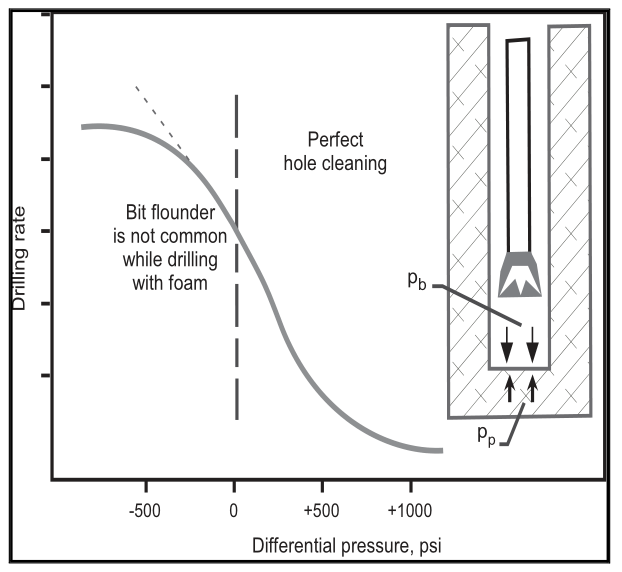
\includegraphics[scale=0.5]{Figs/Fig11.PNG}
		\caption{Tốc độ khoan và áp suất đáy giếng}
	\end{figure}
\subsection{Hạn chế}
	\subsubsection{Giá thành}
	Gaseated drilling thường có giá thành cao hơn so với các phương pháp khoan truyền thống, đặc biệt là khoan ở những vị trí khắc nhiệt như trên biển hay trong sa mạc. So với khoan truyền thống, khoan bằng gaseated fluid còn cần phải có thiết bị kiểm soát khoan xoay, máy nén, bình tách, bình chứa, nhân lực và các chi phí phát sinh trong khi khoan. 
	\subsubsection{Pressure surges}
	Hệ thống gaseated thường không ổn định. Khi pha khí trong dung dịch đi lên tới bề mặt và thoát ra ngoài thông qua đường tiết lưu. Pha lỏng sẽ bị nén xuống dưới làm tăng áp suất đáy giếng và giữ pha khí bên trong cột chất lỏng bị nén. Khi cột dung dịch này được tuần hoàn thông qua đường tiết lưu và làm giảm áp suất trong giếng, quá trình này được lặp đi lặp lại nhiều lần mỗi hai mươi phút tạo ra hiện tượng pressure surges.\par
	Pressure surges thường gây ra những thiệt hại lớn lên thành hệ, làm giảm khả năng ổn định của thành giếng. Hiện tượng này có thể được kiểm soát trong khi khoan bằng cách kết hợp các phương pháp kiểm soát khoan xoay, vận tốc dung dịch, đối áp bề mặt để có thể thay đổi tính chất dòng tuần hoàn ngược.\par
	Ngoài ra, để hạn chế hiện tượng pressure surges tại các vị trí kết nối, có thể bơm thêm khí vào trong giếng trước khi kết nối để làm khô phần trên của cần khoan. Sau quá trình kết nối, phải giảm được khí được bơm vào để có thể loại bỏ pressure surges.
	\begin{figure}
	\centering
	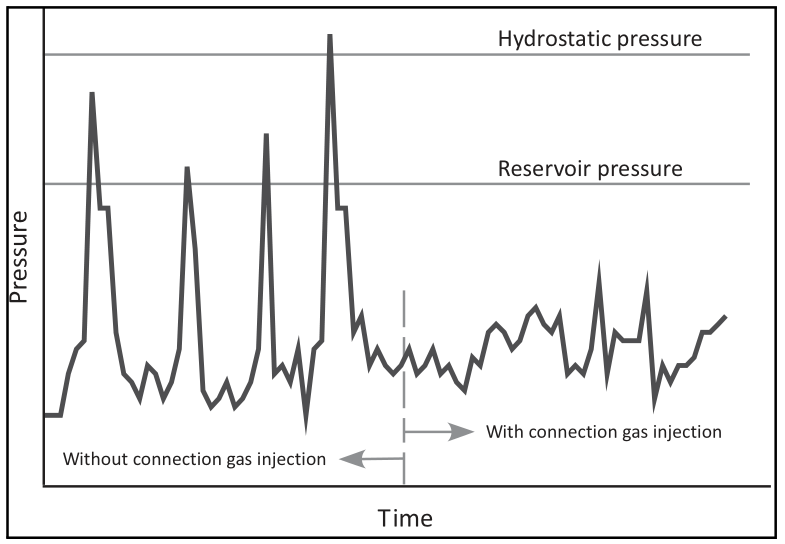
\includegraphics[scale=0.5]{Figs/Fig12.PNG}
	\caption{Tối ưu lượng khí bơm vào hệ thống tuần hoàn trước khi kết nối}
	\end{figure}
	\subsubsection{Một số hạn chế khác}
		\begin{itemize}
			\item Nứt vỡ: Khi xuất hiện những nứt vỡ lớn trong giếng, dung dịch đi vào trong nứt vỡ gây ra hiện tượng mất dòng liên tục ở mức thấp, điều này dễ làm cho giếng bị kick tại những vị trí kết nối. Nguyên nhân chính của vấn đề này là do trọng lực làm thay đổi dòng dung dịch và dòng tuần hoàn khi tắt bơm dung dịch.
			\item Sự hấp thụ: Lực mao dẫn trong vỉa có thể gây ra hiện tương hấp thụ dung dịch khoan, dung dịch bị hút vào trong vỉa kể cả khi giếng đang sử dụng phương pháp khoan dưới cân bằng. Để giảm thiểu lượng dung dịch bị hút vào trong vỉa, áp suất trong khoảng không vành xuyến cần phải nhỏ hơn áp suất thành hệ gây ra bởi áp suất mao dẫn và pha lỏng của dung dịch khoan phải hạn chế được sự dính ướt lên thành hệ.
			\item Ngừng tuần hoàn: Ngừng tuần hoàn có thể dẫn dến hư hại thành hệ hoặc giảm hiệu suất của dung dịch do mất mát dung dịch.
		\end{itemize}
\section{Kỹ thuật Flow-drilling}
\subsection{Tổng quan}
\subsection{Hệ thống thiết bị bề mặt}
\subsection{Kiểm soát đầu xoay}
\subsection{Phương pháp vận hành}
\subsection{Hạn chế của phương pháp}
\end{document}